\documentclass{standalone}
\usepackage{mathpazo}
\usepackage{tikz}

\begin{document}

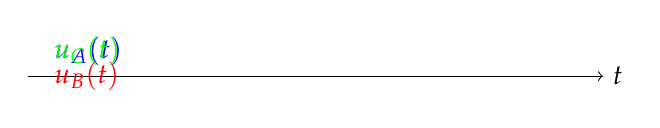
\begin{tikzpicture}[domain = 0:7, samples = 1000]
  % \draw[very thin,color=gray] (-0.1,-1.1) grid (10,1.1);
  \draw[->] (-0.2,0) -- (7.1,0) node[right] {$t$};
  \draw[thick, color=blue] plot[id=Va] function{sin(x)}
  node[above right] {$u_A(t)$};
  \draw[thick, color=red] plot[id=Vb] function{sin(x + 2*pi/3)}
    node[right] {$u_B(t)$};
  \draw[thick, color=green] plot[id=Vc] function{sin(x -2*pi/3)}
  node[above right] {$u_C(t)$};
\end{tikzpicture}

\end{document}


